\documentclass[a4paper,man,natbib]{apa6}

\usepackage[english]{babel}
\usepackage[utf8x]{inputenc}
\usepackage{graphicx}
\usepackage[colorinlistoftodos]{todonotes}
\usepackage{amsmath,amsfonts,mathabx}
\usepackage{epigraph}
\usepackage[figuresright]{rotating}
%\usepackage[ansinew]{inputenc}
\usepackage{multirow}
%\setmainfont{Times New Roman} 
%\setsansfont{Times New Roman} 
%\setmonofont{Times New Roman} 
% Keywords command

\newcommand{\cmmnt}[1]{\ignorespaces}

\providecommand{\keywords}[1]
{
  \textbf{\textit{Keywords---}} #1
}
\usepackage[doublespacing]{setspace}

\setlength\epigraphwidth{.8\textwidth}

\title{The Discrete Metric in Categorization Under Time Pressure}
% Effect of Time Pressure on Distance Metrics in Categorization
\shorttitle{Discrete Metric Under Time Pressure}
\author{Florian I. Seitz}
\affiliation{University of Basel}

\abstract{The generalized context model \citep{nosofsky1986attention}, which excels at explaining human categorization behavior, assumes the Minkowski metric to represent psychological distance. I propose that in categorization under time pressure people compute psychological distance heuristically with the discrete metric which counts the number of non-identical feature values. 
61 psychology students (43 females, $M_{age}$ = 24.13 years, age range: 19--50 years) from the University of Basel acquired in the learning phase the category structure of eight stimuli with three quarternary features by trial--by--trial supervised category learning. After meeting the accuracy criterion participants categorized six novel and four old stimuli 14 times without feedback in the test phase. We applied time pressure to a random half of participants in the test phase.
Inferential tests at the aggregate level showed that pressure the Minkowski metric could account for participants' categorization behavior both with and without time (\textit{p} < .001, respectively). Cognitive modeling yielded that the discrete metric with attention centered on all features in the condition without time pressure and a random choice model in the condition with time pressure outperformed the other models both on the aggregate and on the individual level.
The present findings suggest that the discrete may not apply to people in speeded categorization situations but to a substantial amount of people in categorization without time pressure. We compare these findings to a potential rule--based model and point out potential differences in cognitive processing when categorizing stimuli with known versus unknown feature values.} 

\keywords{categorization, time pressure, Minkowski metric, discrete metric, distance}

\begin{document}
\maketitle

%\vspace*{\fill}
\epigraph{There is nothing more basic than categorization to our thought, perception, action, and speech. [...] An understanding of how we categorize is central to any understanding of how we think and how we function, and therefore central to an understanding of what makes us human.}{George Lakoff, 1987, pp.5--6}

Humans frequently engage and excel in categorization---the generation and identification of groups from a bigger amount of objects \citep{nosofsky1986attention}---which is thus considered one of the most fundamental cognitive phenomena overall \citep{ashby2001categorization, bruner1956study, cohen2005bridging, lakoff1987women, goldstone2003concepts}. Past research has uncovered a wide scope of factors relevant to categorization such as the strategies and models people used during categorization learning and generalization \citep[for an overview over the diverse models of categorization, see][]{kruschke2008models,wills2013models}. One finding from these studies is that people first rely on simple categorization strategies and only if necessary pass on to more complex strategies \citep{gluck2002people, meeter2006strategies, meeter2008probabilistic, johansen2002there, smith1998prototypes}. Strategy simplification, however, has not been central in research on speeded categorization, albeit that under time pressure the need for simplifying the categorization process might be particularly pronounced. In contrast, speeded categorization research has focused on sequential information sampling such as competing retrieval of comparison objects from memory \citep{nosofsky1997exemplar, nosofsky1999effects, nosofsky2005speeded} or sequential processing of features (\citealp{lamberts1995categorization, lamberts1998time, lamberts2000information}; for a combination of both processes, see \citealp{cohen2003extension}). 

Strategies can be held simple notably by a reduction of the number of processed features leading in an extreme case to a unidimensional strategy where categorization behavior depends only on one single feature \citep{johansen2002there} and by the use of a central tendency instead of multiple actual instances to represent a category \citep{smith1998prototypes}. % While evidence suggests that people reduce the number of instances they compare an object to classify to and base this comparison on a smaller amount of features
However, in tasks where computation ability is lacking, the comparison itself may also be held simple by checking identity of two objects' values on a given feature leading to binary differences rather than generally assumed metric differences. The present thesis tests this hypothesis in a speeded categorization task with an experimental design that optimally discriminates between the metrical and binary difference computation while allowing as well to test for the alternative strategy simplification of unidimensional strategies.
% Throughout this research, it was generally assumed that people compare objects metrically such that larger feature value differences between objects result in lower similarity between these objects. In tasks where computation ability is lacking people might compare objects more heuristically by checking identity of the values on a given feature. 

\iffalse
Categorization refers to the partitioning of objects into a smaller amount of groups with distinct responses where each group is associated with a unique response \citep{cohen2005bridging, nosofsky1986attention, nosofsky1989further}. As people categorize countless times throughout their life, the mental process of grouping objects into categories is considered to be one of the most fundamental cognitive phenomena overall \citep{ashby2001categorization, bruner1956study, cohen2005bridging, lakoff1987women, goldstone2003concepts} and thus has received substantial attention in scientific research. From the late 70s on, numerous cognitive models have been established which try to describe how people perform categorizations \citep[for an overview over the diverse models of categorization, see][]{kruschke2008models,wills2013models}. The present thesis analyzes an especially popular categorization model---the generalized context model \citep{nosofsky1984choice, nosofsky1986attention, nosofsky2011generalized}. The generalized context model is defined as an exemplar--based model, where people retrieve instances from memory (i.e., exemplars) and compare them with an instance to categorize \citep[i.e., the probe;][]{medin1978context}. Comparisons between probe and exemplars are expressed as distances which in turn are used to predict category membership. Exemplar-based models of categorization may be distinguished from prototype-based models of categorization, which assume the retrieval of each category's central tendency instead of individual exemplars \citep{reed1972pattern, smith1997straight, smith1998prototypes}. 

In the following parts of this introduction, I will describe and review the generalized context model. Then, I will argue that people might use a binary measure of distance, the discrete metric, when confronted with time pressure during categorization. Differences between the generalized context model implemented with the usual distance metric and the one implemented with the discrete distance will be discussed before presenting the study which aimed to test against each other these two models in a categorization task with time pressure.
\fi

\subsection{Theoretical Background: Categorization under Time Pressure}


\subsection{Formal Models: The Generalized Context Model With two Distance Metrics}
The generalized context model \citep{nosofsky1986attention} is an exemplar--based model, where people retrieve instances from memory (i.e., exemplars) and compare them with an instance to categorize \citep[i.e., the probe;][]{medin1978context}. People are assumed to represent each exemplar as a point in a multidimensional space where the exemplar's feature values are the point's coordinates. Comparisons between probe and exemplars are expressed as distances, which can be interpreted as how far away the probe is spatially positioned from the exemplar of comparison. Distances are then transformed into similarities, such that high distances correspond to low similarities and low distances to high similarities. Finally, the aggregate similarity of the probe to all exemplars of one category relative to the aggregate similarity to all exemplars states the model's category membership prediction for the probe. The higher the similarity of the probe to the exemplars of one category the higher the model's prediction of assigning the probe into this very category. 

In the following, I will describe the three computational steps of distance, similarity, and categorization probability which the generalized context model assumes in a multidimensional, multivalued stimulus space with two categories. The formalization of the model is equivalent to \cite[][pp.281--282]{nosofsky1989further}, except that it has been generalized to more than two dimensions. 

\subsubsection{Categorization probability}
The generalized context model \citep{nosofsky1989further} predicts a probe's categorization probability by means of the similarity between the probe and the categories to choose from. Specifically, the probability with which probe $i$ is categorized into category $A$ is defined as 
\begin{equation}
P(R_{A}|i) = \frac{b_{A}\sum\limits_{j \in A} s_{ij}}{b_{A}\sum\limits_{j \in A} s_{ij} + (1 - b_{A})\sum\limits_{k \in B} s_{ik}},
\end{equation}
where $P(R_{A}|i)$ is the probability of rendering response $A$ given probe $i$, $s_{ij}$ is the similarity between probe $i$ and exemplar $j$, and $b_{A}$ is the response bias for category $A$. The function is derived from the similarity--choice model for stimulus identification \citep{luce1963detection, shepard1957stimulus} and bases categorization probability on the share of the aggregate similarity to both categories that is attributable to one of the two categories.

\subsubsection{Similarity}
The similarity $s_{ij}$ between probe $i$ and exemplar $j$, in turn, is computed from the distance of the two objects in a multidimensional space. The transformation of distance into similarity is given by Shepard's universal law of generalization \citep{shepard1987toward}
\begin{equation}
s_{ij} = \exp\left(-c*d_{ij}^p\right),
\end{equation}
where $d_{ij}$ is the distance between probe $i$ and exemplar $j$, $c$ (with $0 \leq c$) is an overall sensitivity parameter, and $p$ is a parameter that determines how similarity relates to psychological distance. Popular instances of the similarity function are the exponential decay function ($p = 1$) for discriminable stimuli and the Gaussian function ($p = 2$) for confusable stimuli \citep{ennis1988confusable, nosofsky1985luce}. The sensitivity parameter $c$ describes the convexity of the similarity function indicating thus the steepness with which similarity decreases as distance increases. For high values of $c$, similarities are already low at very small distances already. For low values of $c$, similarities are still high at very large distances. In both cases, the model doesn't discriminate between different distances. The parameter $c$ thus denotes a person's sensitivity to psychological distance.

\subsubsection{Distance}
The generalized context model calculates distances between the probe and the previously encountered exemplars which have been retrieved from memory by means of the Minkowski distance. The Minkowski distance is a geometric distance function (also named metric), formally given as 
\begin{equation}
d_{ij} = \left[\sum\limits_{m=1}^M w_{m}*\mid x_{im} - x_{jm}\mid ^r\right]^\frac{1}{r},
\end{equation}
where $d_{ij}$ is the Minkowski distance between probe $i$ and exemplar $j$, $x_{im}$ is the value of probe $i$ on feature $m$, $w_{m}$ is the attention weight attributed to feature $m$ (with $0 \leq w_{m} \leq 1$ and $\sum w_{m} = 1$), $M$ is the number of features, and $r$ describes the form of the distance metric (with $r >= 1$). Popular instances of the Minkowski distance are the Manhattan distance ($r = 1$) for highly separable-feature stimuli and the Euclidean distance ($r = 2$, a generalized form of the Pythagorean theorem for $M$ features) for integral-feature stimuli \citep{shepard1964attention, nosofsky1986attention, garner1974processing}. With increasing $r$ the resulting distance between a given probe and a given exemplar cannot increase and absolute differences between distances to different exemplars are reduced. Values of $r$ are constrained to be equal to or higher than 1 for adherence with the triangle inequality, a prerequisite of geometric distance metrics \citep{jakel2008similarity,francois2007concentration,tversky1982similarity,beals1968foundations}. The triangle inequality states that in each triangle the sum of two sides must be at least as great as the remaining side. For the Minkowski metric this means that the sum of all feature--wise distances between probe and exemplar must be greater than the distance between the instances across features. This prerequisite is violated for $r < 1$ and in such a case the Minkowski distance is not anymore a metric \citep[][p. 5]{kress1989linear}. 

Whereas the generalized context model and related models of categorization assume people to compute Minkowski distances between the probe and the exemplars, an inexhaustible pool of further metrics exist that could potentially model how people represent psychological distance. In fact, the only prerequisites that metrics need to meet are (a) the non--negativity axiom (all distances are 0 or higher), (b) the identity of indiscernibles (distances between identical objects are 0), (c) symmetry (the distance between two objects is independent of the order of the objects), and (d) the triangle inequality discussed above \citep{restle1959metric}. The discrete distance is one such possible metric, given by 
\begin{equation}
\rho_{m}(x_{im}, x_{jm}) = 
\begin{cases}
	1 & x_{im} \neq x_{jm} \\
	0 & else 
\end{cases},
\end{equation}

where $\rho_{m}(x_{im}, x_{jm})$ is the discrete distance function between the two exemplars $x_{im}$ and $x_{jm}$. In the generalized context model, this yields

\begin{equation}
d_{ij} = \left[\sum\limits_{m=1}^M w_{m}* \rho_{m}(x_{im}, x_{jm}) ^r\right]^\frac{1}{r}.
\end{equation}

%To Do: Write that Minkowski is geometric (cite Goldstone for other similarity calculations) and then write below that geometric models with r < 1 don't fulfill the triangle inequality axiom.

\subsubsection{Relation to unidimensional generalized context model versions}
Instead of using the heuristical discrete metric to simplify categorization under time pressure, people might as well base their categorization behavior on fewer stimulus features. In an extreme case, participants only attend to one feature, probably the feature they deem most relevant, and categorize a probe only based on this single feature. In the generalized context model \citep{nosofsky1989further} attention partition across features is given by the attention weights $w$s. Whereas in the multidimensional generalized context model attention weights are only constrained to be positive and to sum up to 1, in the unidimensional generalized context model one of the attention weights is set to 1 and the remaining to 0. In a given environment, there exist as many unidimensional generalized context model versions as the stimulus contains features. An important distinction between the unidimensinoal and the multidimensional generalized context model is that the former cannot model feature interactions as only one feature is attended to. In cases where people have to attend to multiple features in order to learn a category structure, such as in a non--linearly separable design as used in this study, the lowered computational demands which the use of the unidimensional generalized context model provides might be outweighed by the poor categorization accuracy. I thus hypothesize that the generalized context model with the discrete metric outperforms the unidimensional model with the Minkowski metric. I further implemented the unidimensional generalized context model with the discrete metric which needs the least computational power as both the distance metric is simplified and less features are processed. In case this model describes a participant this is counted as evidence for the discrete metric as the primary aim of this thesis is to analyze whether people use different distance metrics in conditions with time pressure and without time pressure.
 
\subsubsection{Relation to prototype models}
The generalized context model, which assumes people to rely on actual instances experienced in the past to represent categories \citep{medin1978context, nosofsky1986attention}, diverges in this assumption of category representation from other existing approaches where categories are represented by abstract central tendencies (i.e., prototypes; \citealp{posner1968genesis}). In these prototype--based models, a given probe is compared to the categories' prototypes instead of to the categories' exemplars \citep{nosofsky1987attention}. % The difference between exemplar--based and prototype--based categorization models thus occurs during the distance computation as different category representatives are being compared to the probe (i.e., exemplars or prototypes). 
Due to the very fine--grained representation of categories using actual experienced instances, the categorization predictions of the generalized context model are sensitive to influences from individual exemplars---influences which are absent in prototype models \citep{nosofsky2011generalized, nosofsky1992exemplars, medin1978context}. Following a long debate of whether people represent categories using prototypes or exemplars, research indicates that exemplar-based categorization models using a non--linear similarity rule, such as the generalized context model, outperform prototype models in explaining participants' categorization behavior (\citealp{nosofsky1992exemplars}, see also \citealp{scholkopf2002learning}). However, further evidence indicates that people shift from a prototype--based model during early categorization to a computationally more complex exemplar--based model as the number of experienced exemplars increases (\citealp{smith1998prototypes}, but for an alternative view, see \citealp{nosofsky2002exemplar}). Albeit the use of prototypes is computationally less challenging than the retrieval of actual exemplars, I didn't integrate a prototype--based model, as design optimization revealed that no design simultaneously may recover and discriminate the two distance metrics (i.e., the Minkowski and the discrete metric) and the two types of category representation (i.e., prototypes and exemplars). Furthermore, in the present study, participants had to learn the category membership of only a few stimuli in a non--linearly separable category structure---two design properties for which literature suggests the use of exemplar--based strategies instead of prototype--based strategies \citep{smith1998prototypes, smith2000thirty}. Hence, I assume for the categorization task of the present study that people use an exemplar--based model, namely the well--established generalized context model \citep{nosofsky1986attention}.

\subsection{Hypotheses}
The present thesis analyzes whether people use different distance metrics in conditions with and without time pressure. Specifically, given the generalized context model \citep{nosofsky1989further}, I expect people to use the well--established multidimensional Minkowski metric in the baseline condition without time pressure and the heuristical discrete metric (either unidimensional or multidimensional) in the condition with time pressure. Based on this main hypothesis, I state the following specific hypotheses which all presuppose the use of the generalized context model: 

Under time pressure, people use the discrete metric (H1a), else a unidimensional Minkowski metric (H1b), else the multidimensional Minkowski metric (H1c). Across participants, the multidimensional and the unidimensional discrete metric outperform the remaining models in predicting participant behavior, followed by the unidimensional Minkowski metric on the second rank, the multidimensional Minkowski metric on the third rank, and the random choice model on the final rank (H1d). At the individual level, the multidimensional and the unidimensional discrete metric describe more participants than any of the remaining models (H1e). Furthermore, at the individual level, the count of participants best described by each models follows the rank order layed out in H1d (H1f). 

Without time pressure, people use the multidimensional Minkowski metric, but not the unidimensional nor the multidimensional discrete metric (H2a). Across participants, the multidimensional Minkowski metric outperforms the remaining models, while the random choice model is inferior to all remaining models in predicting participant behavior (H2b). I have no hypotheses about the relative performance amongst the unidimensional Minkowski metric, the unidimensional discrete metric, and the multidimensional discrete metric. At the individual level, the multidimensional Minkowski metric describes more participants than any of the remaining models and the count of participants best described by each model follows the rank order of H2b (H2c). 

Finally, the multidimensional discrete metric describe more participants with time pressure than without time pressure (H3a), whereas the multidimensional Minkowski metric describes more participants without time pressure than with time pressure (H3b).

\section{Method}

\subsection{Optimal Experimental Design}
An optimal experimental design is defined as a design with ``the greatest likelihood of differentiating the models under consideration'' \cite[][p. 500]{myung2009optimal}. Being able to differentiate between the different models under consideration means that each model is associated with unique behavioral predictions. Participant behavior can thus be linked with greater certainty to one of the models under consideration. Furthermore, through the maximization of model prediction differences, design optimization increases model recovery (i.e., the model underlying the data is found to be the best-fitting model as well). The advantages of design optimization are thus two-fold: A participant's behavior can be associated more exclusively with one of the models under consideration and the odds are higher that this best-fitting model is the model that was used by the participant to generate her responses \citep[albeit that each scientific model is only an approximation of the participant's cognitive model; see][]{myung2009optimal}. Design optimization maximizes thus the experiment's degree of informativeness and cost-effectiveness by improving the design while keeping the necessary sample and trial size at a low level \citep{cavagnaro2009better, ouyang2016practical, raffert2012optimally, atkinson2007optimum, nelson2005finding}. 

The advantages of design optimization are most pronounced when the different models differ quantitatively instead of qualitatively as well as when several variables have to be considered simultaneously during the designing process of the experiment making thus a good design hardly visible to the naked eye \citep{myung2009optimal}. Both criteria apply for categorization studies.
% First, categorization models with a Minkowski metric vs. a discrete metric differ in their predicted probabilities of assigning a given stimulus into one of two categories. Second, the experimental design includes many variables to consider, such as which stimuli to include in either learning or test set and within the learning set how the stimuli are assigned to the two categories. 
The potential of optimal experimental design is shown in a reanalysis of the designs of the first two experiments of \cite{smith1998prototypes} which aimed at distinguishing the generlized context model \citep{nosofsky1986attention} from the multiplicative prototype model \citep{smith1998prototypes} by using six-dimensional binary stimuli \citep{myung2009optimal}. Even though the best experimental design used in \cite{smith1998prototypes} had a high model recovery of 88.8\%, the optimal design that was possible yielded a model recovery rate of 96.3\%, minimizing thus the risk of a model fitting error by eight percent.  

In the light of these findings, we ran simulations to find a categorization environment such that the discrete metric and the Minkowski metric implemented in the generalized context model can be optimally discriminated given the responses during the test phase, in the expectation.\footnote{In the first simulations we further wanted to discriminate the generalized context model from the multiplicative prototype model. However, as simultaneously discriminating the two models and the two distance metrics led to insufficient model recovery rates, we dropped the multiplicative prototype model from the remaining simulation analyses} The simulations were chronologically iterated over (a) the design (i.e., all possible category structures with equal category base rates for all subsets of eight of 64 stimuli in the learning phase, under the constraint that learning stimuli differ from each other maximally by 1 unit per feature to ensure that the discrete and the Minkowski metric yield identical distances and thus none is favored by the learning phase design), (b) the true model (i.e., the generalized context model with either the Minkowski metric or the discrete metric), (c) the true parameter combination (i.e., attention weights \textit{w}'s ranging from $0$ to $1$ in steps of $1/3$ and the overall sensitivity parameter \textit{c} ranging from $0.1$ to $4.1$ in steps of $1$; the decay parameter \textit{p} and the parameter defining the distance metric \textit{r} were fixed to 1), and (d) the fitting model (i.e., the generalized context model with either the Minkowski metric or the discrete metric).

% Out of the 64 possible stimuli we predefined to have eight stimuli in the learning set (i.e., four in each category). Not counting exactly inversed and thus repetitive partitioning of learning stimuli into the two categories (e.g., stimuli 1--4 in category A and stimuli 5--8 in category B vs. stimuli 1--4 in category B and stimuli 5--8 in category A) this yields $\dfrac{64!}{56!*8!}*\dfrac{8!}{8!*4!*2} = 154,915,787,880$ possible designs. As this would lead the simulations to last very long, we restricted the design space to include only designs in which all stimuli had on each dimension maximally a city-block distance of 1 to each other. This restriction at the same time minimized the risk of biasing participants towards one of the models in the learning phase as the distances resulting from value ranges of 1 are the same for the Minkowski and the discrete metric and leads to a more approachable number of 140 possible designs.

For a given design, true model, and true parameter combination we simulated binary participant responses (i.e., category A or B) based on the true model's predictions for the learning set which was replicated 20 times and for the test set (i.e., the stimuli that were not part of the learning stimuli) which was replicated 10 times. Then, the free parameters (i.e., attention weights and the overall sensitivity parameter) of both models were fitted to the simulated data of the learning set excluding the first eight uninformative trials\cmmnt{ where models have not encountered enough instances to render informative predictions} and fixed to the resulting optimal parameters for each participant. Next, predictions for the test set were computed with every model and the log likelihood between the simulated participant responses under the true model and the predictions of each fitting model was calculated for the test phase data. This procedure allowed conducting model recoveries for every design across all permissible parameter combinations. The best design was the design for which the winning model recovered the true data--simulating model best, across the permissible model parameters. In the best design, the learning criterion was met by both models when adding a softmax choice rule. From the 56 stimuli in the test phase of the best design, the six stimuli that discriminated models best were selected. Figure \ref{fig:environment} shows the stimuli in the resulting design.

\subsubsection{Model Recovery}
The generalized context model with the discrete metric was correctly recovered in 100\% of all cases, the generalized context model with the Minkowski metric was correctly recovered in 86.7\% \textbf{(I have to recheck this)} of all cases. 

\subsection{Materials and Design}
The experiment was conducted on \textit{computers} and programmed in Expyriment \citep{krause2014expyriment}.  Participants classified different products (i.e. stimuli) into brand L or brand R (i.e., categories) by pressing the left and right arrow key, respectively. Products were based on the material of \cite{albrechtxxxunstacking}. Each product consisted of the same three ingredients (i.e., features) represented by grey beams with one to four quantity units of each ingredient (i.e., feature values) represented by colored squares. Figure \textit{ref} illustrates the material. Participants learned the category structure of eight stimuli in the learning phase, and categorized four of them and six novel stimuli in the test phase. Figure \ref{fig:environment} illustrates the learning set and the test set environment and Table \ref{tab:environment} shows the median model predictions for all stimuli of the learning set and the test set. Brand name and the corresponding correct arrow key as well as the distribution of the features to the three grey beams and the three colors of the stimuli were randomized across participants.

\begin{figure}[htbp]
\centering
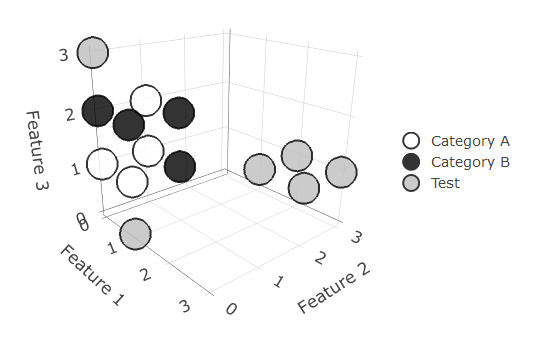
\includegraphics[width = \textwidth]{fig_environment.png}
\caption{Learning stimuli (in black and white) including their category structure and test stimuli (in grey). Each axis of the graph represents one feature, and the coordinates of each sphere represent the feature values of the respective stimulus. Stimuli in the learning phase include all learning stimuli, stimuli in the test phase include all test stimuli as well as the learning stimuli 002, 012, 101, and 111.}
\label{fig:environment}
\end{figure}

\begin{sidewaystable}
\begin{center}
\begin{threeparttable}
\caption{Environment used and median model predictions}
\label{tab:environment}
\begin{tabular}{cccccccccc}
\toprule
 &  & \multicolumn{4}{c}{Discrete} & \multicolumn{4}{c}{Minkowski} \\
\cmidrule(r){3-6} \cmidrule(r){7-10}
 &  & \multicolumn{1}{c}{Multidimensional} & \multicolumn{3}{c}{Unidimensional} & \multicolumn{1}{c}{Multidimensional} & \multicolumn{3}{c}{Unidimensional} \\
\cmidrule(r){4-6} \cmidrule(r){8-10}
Stimulus & \multicolumn{1}{c}{Category} &  & \multicolumn{1}{c}{\textit{w}_1 = 1} & \multicolumn{1}{c}{\textit{w}_2 = 1} & \multicolumn{1}{c}{\textit{w}_3 = 1} &  & \multicolumn{1}{c}{\textit{w}_1 = 1} & \multicolumn{1}{c}{\textit{w}_2 = 1} & \multicolumn{1}{c}{\textit{w}_3 = 1}\\
\midrule
\addlinespace
\multicolumn{2}{c}{\emph{Learning phase}} \\
\addlinespace
001 & B & 0.97 & 0.74 & 0.50 & 0.74 & 0.97 & 0.74 & 0.50 & 0.74\\
002\makebox[0pt][l]{$^{\ast}$} & A & 0.09 & 0.74 & 0.50 & 0.26 & 0.09 & 0.74 & 0.50 & 0.26\\
011 & B & 0.99 & 0.74 & 0.50 & 0.74 & 0.99 & 0.74 & 0.50 & 0.74\\
012\makebox[0pt][l]{$^{\ast}$} & B & 0.93 & 0.74 & 0.50 & 0.26 & 0.93 & 0.74 & 0.50 & 0.26\\
101\makebox[0pt][l]{$^{\ast}$} & B & 0.91 & 0.26 & 0.50 & 0.74 & 0.91 & 0.26 & 0.50 & 0.74\\
102 & A & 0.03 & 0.26 & 0.50 & 0.26 & 0.03 & 0.26 & 0.50 & 0.26\\
111\makebox[0pt][l]{$^{\ast}$} & A & 0.07 & 0.26 & 0.50 & 0.74 & 0.07 & 0.26 & 0.50 & 0.74\\
112 & A & 0.01 & 0.26 & 0.50 & 0.26 & 0.01 & 0.26 & 0.50 & 0.26\\
\midrule
\addlinespace
\multicolumn{2}{c}{\emph{Test phase}} \\
\addlinespace
003 & - & 0.63 & 0.74 & 0.50 & 0.50 & 0.09 & 0.74 & 0.50 & 0.26\\
100 & - & 0.37 & 0.26 & 0.50 & 0.50 & 0.91 & 0.26 & 0.50 & 0.74\\
221 & - & 0.85 & 0.50 & 0.50 & 0.74 & 0.07 & 0.26 & 0.50 & 0.74\\
231 & - & 0.85 & 0.50 & 0.50 & 0.74 & 0.07 & 0.26 & 0.50 & 0.74\\
321 & - & 0.85 & 0.50 & 0.50 & 0.74 & 0.07 & 0.26 & 0.50 & 0.74\\
331 & - & 0.85 & 0.50 & 0.50 & 0.74 & 0.07 & 0.26 & 0.50 & 0.74\\
\bottomrule
\addlinespace
\end{tabular}
\begin{tablenotes}[para]
\textit{Note.} Median model predictions for the stimuli used in the learning phase and the test phase. The four stimuli from the learning phase marked with an asterisk also appeared in the test phase.
\end{tablenotes}
\end{threeparttable}
\end{center}
\end{sidewaystable}

Participants' main task was to categorize products into two brands. The dependent variable was the pressed key which represented the product's assumed brand. The independent variable was the time pressure induced to a random half of participants in the test phase. It allowed a participant 400 milliseconds plus 30\% of the median decision time needed by this participant across the final 100 learning trials. The study had thus a repeated--measures 2x1 between--subjects design. Further variables assessed were response times per trial and the amount of time pressure if any.

\subsection{Participants}
Sixty-one psychology students (43 females, $M_{age}$ = 24.13 years, $SD_{age}$ = 6.39 years, age range: 19--50 years) from the University of Basel were recruited over an online platform of the Faculty of Psychology to participate in a categorization study. All participants had a high--school or a higher degree and were asked for color blindness, visual impairment, and in case of impaired vision whether they carried a visual aid during the experiment. Participants selected themselves into the sample and there were no inclusion criteria. Up to six participants could show up to the same experimental session. Participant data were listwise deleted if the participant failed to reach the accuracy criterion in the learning phase within an hour, answered ''absolutely unclear'' or ''somewhat unclear'' to the question if the task in the experiment was clear or in the time pressure condition exceeded the time limit in more than 50\% of the test trials for a given test stimulus and in the no time pressure condition had a log transformed reaction time more than three standard deviations below the mean of the log transformed reaction times of the learning phase in more than 50\% of the test trials for a given test stimulus.  As a compensation for study participation participants received course credit proportionally to the amount of time needed to complete the study. Eight additional subjects participated in the study but had to be excluded from the analyses as they reported that the task was somewhat or absolutely unclear to them, two participants failed to reach the accuracy criterion, and two participants' data were used for pretesting purposes.

Sample size was predetermined by a model--based power simulation. Across participants the true probability of choosing the Minkowski metric changed from 70\% to 30\% and the true probability of choosing the discrete metric changed from 30\% to 70\% when time pressure was introduced. For every participant, a random combination of parameters that met the accuracy criterion was sampled for the two model versions, respectively, and a discrete metric weight was sampled from a normal distribution truncated between 0 and 1 with the mean being equal to the share of participants using the discrete metric in the respective time pressure condition and SD =  .3. For any given test phase trial the discrete metric weight indicated how much the predictions of the discrete model version influenced the probabilities underlying simulated participant responses relatively to the predictions of the Minkowski model version. The log likelihood of the simulated responses was calculated for both model versions on the participant level and transformed into Akaike weights \citep{wagenmakers2004aic}. A given model was accepted if its Akaike weight exceeded .95. One--sided two proportion z--tests were calculated for every sample size comparing the proportion of accepted discrete model versions with time pressure and without time pressure. Figure \ref{fig:power} illustrates the proportion of significant results for every sample sizes across 1000 iterations. Given an aspired power of .8, a total sample size of N = 60 (n = 30 in each condition) was necessary to achieve 89\% power. The final sample included 31 participants without time pressure and 30 participants with time pressure.

\begin{figure}[htbp]
\centering
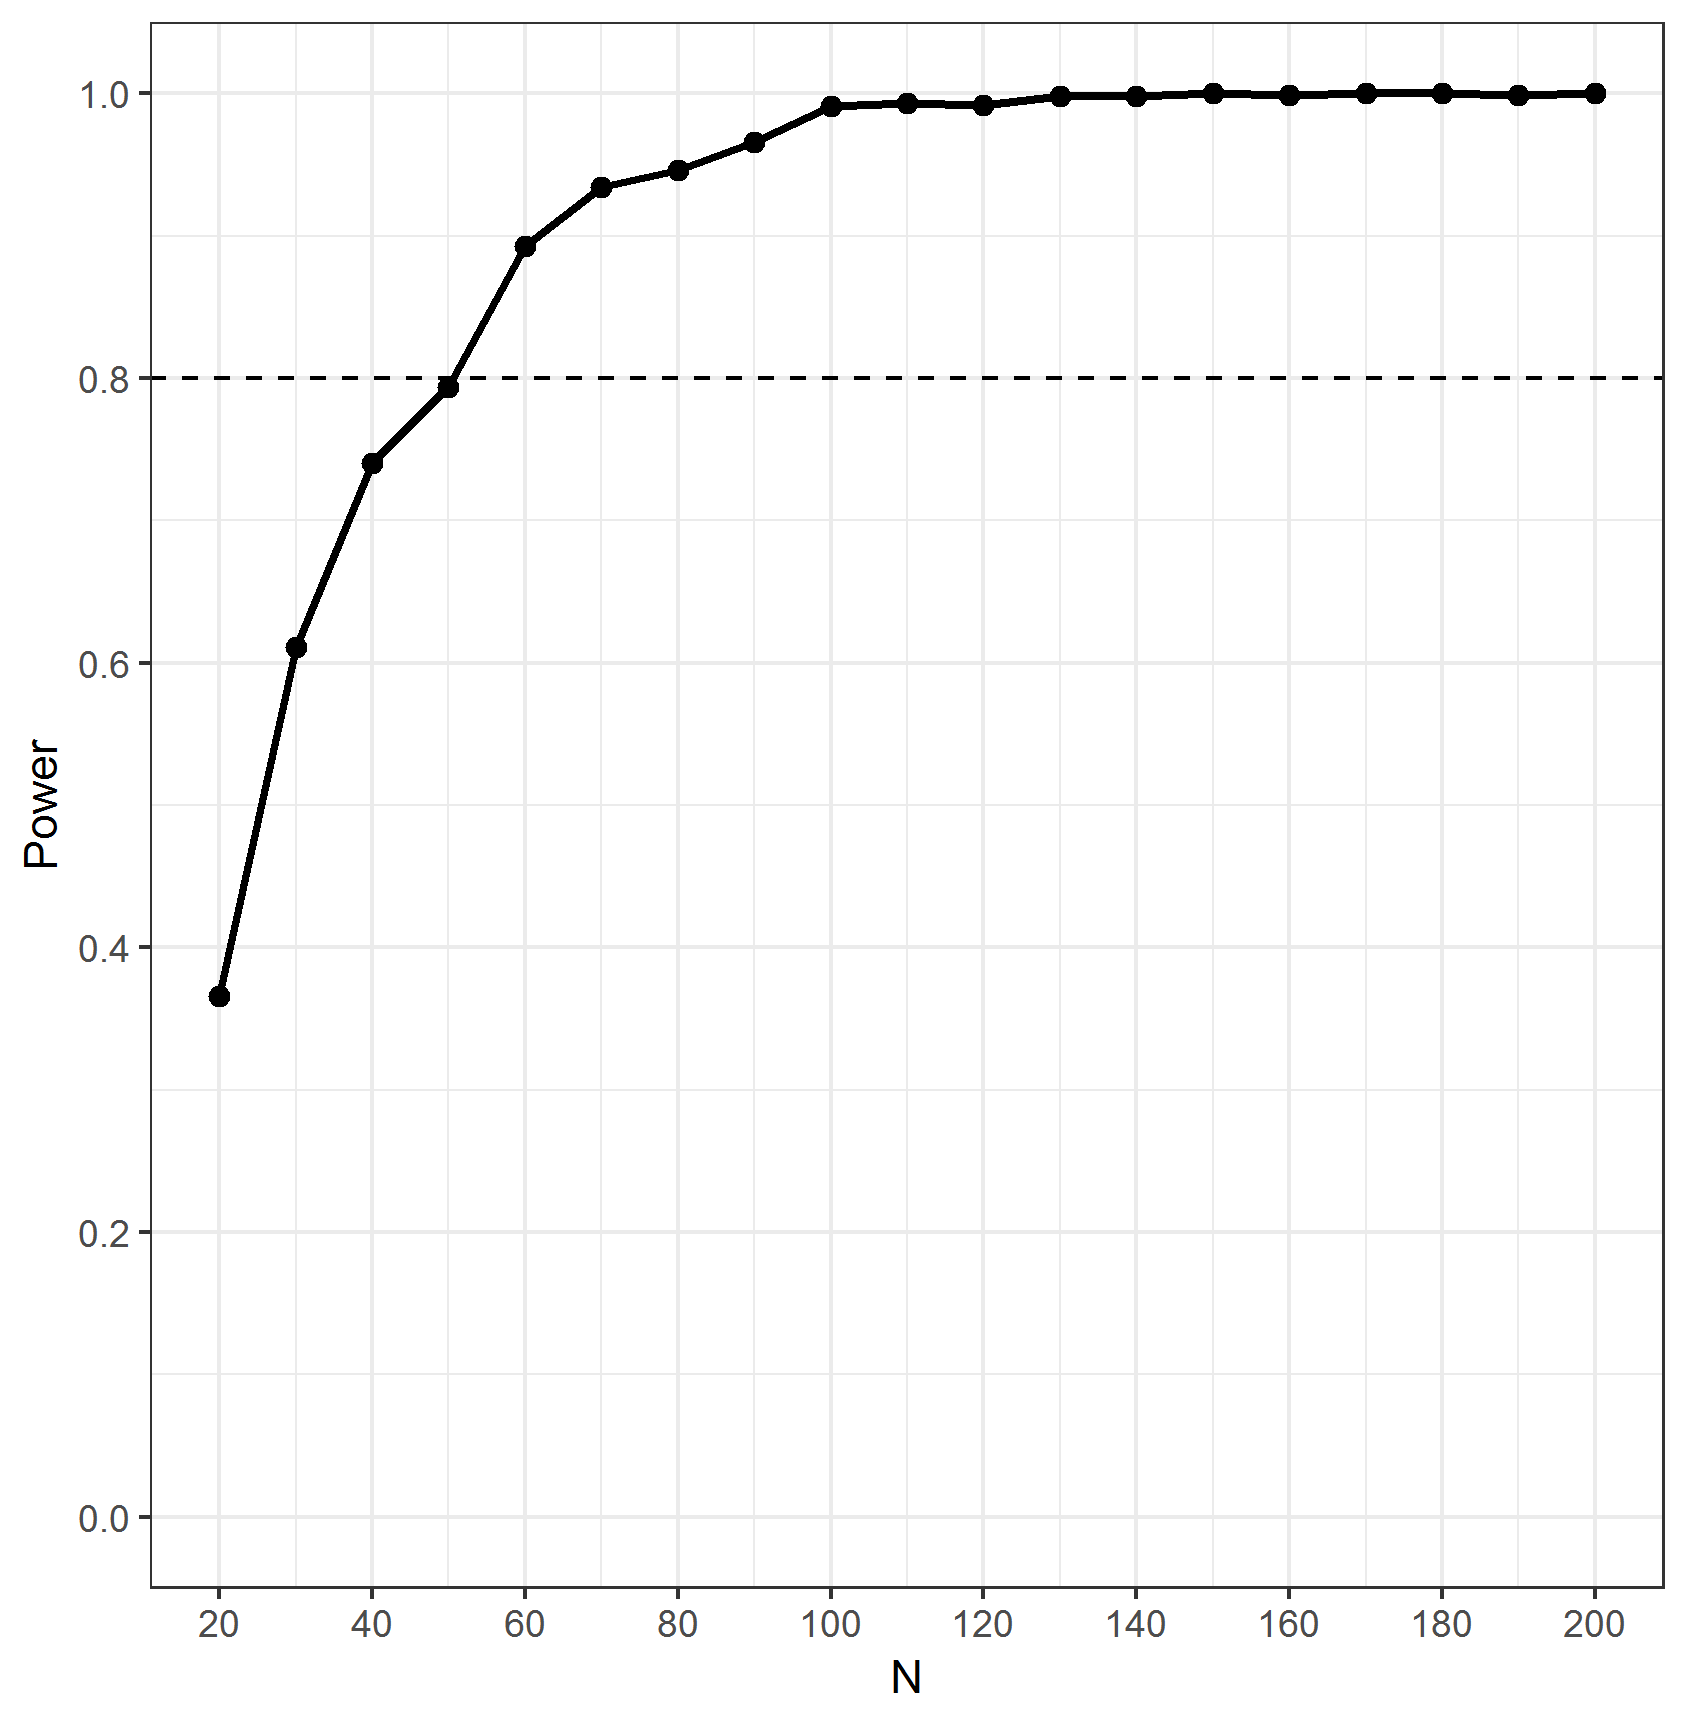
\includegraphics[width = \textwidth]{fig_power.png}
\caption{Power in dependence of sample size N. Power estimation was based on a model--based power simulation where the true probability of using the Minkowski metric changed from 70\% to 30\% and the true probability of using the discrete metric changed from 30\% to 70\% when time pressure was introduced. To achieve the aspired power of .8, 60 participants (n=30 in each condition) were needed.}
\label{fig:power}
\end{figure}

\subsection{Procedure}
After arriving at computer laboratory of the Center of Economic Psychology, participants were greeted, seated in front of a computer which was delimited from the other computers by dividing walls, and were provided with an informed consent which they could read through and sign in case of agreement. Upon signature, the experimenter typed in the participant id to start the experiment and the participant was presented a series of instructions on the computer (for the exact instructions, see \textit{appendix}. Participants first read, that they had to learn to assign different products to two different brands (brand L and brand R), that each product consisted of the same three ingredients but differed from other products in the specific ingredient quantities. They then saw a randomly chosen product (see Figure \textit{ref} for an example), read that each grey beam represented one ingredient and the number of colored squares in the beams indicated the quantity of the respective ingredient. To familiarize with the products, participants then had to click on each ingredient ten times. With each click the quantity of the respective ingredient increased or decreased by one unit, ensuring that all participants saw all possible values on each feature. Participants then read that in each trial they would be presented with a random chosen product and their task was to correctly guess the brand of the respective product by pressing the left and right arrow keys. Participants read that the experiment consisted of two phases: In the first phase, they would learn the correct brand of each product and receive feedback after entering their answer. After achieving to consistently assign the products to the correct brand, they would reach the second phase and have to assign again several products to the brand to which they belonged most likely without receiving feedback. Participants in the time pressure condition furthermore read that they would have a time limit for their response in the second phase which they shouldn't exceed.

\subsubsection{Learning phase}
In the learning phase participants learned the category structure of eight products. All blocks of the learning phase included each of the eight products; the sequence within each block was randomized. In every trial participants could look at the given product for as long as they wished. Participants could then assign the product to brand L or R by pressing the left and right arrow key, respectively. Depending on the correctness of their response, participants received feedback in form of a joyous, green smiley and the exclamation ''Correct!'' or in form of a sad, red smiley and the exclamation ''False!'' if their response was incorrect. Participants could continue looking at the product and the feedback for as long as they wished and then proceed to the next trial by pressing the upper arrow key. In case an invalid key was pressed, participants were reminded which keys to press to assign the product to a brand and to continue to the next trial. After the first 100 learning trials participants received every 50 trials feedback of their accuracy in the last 100 trials. Participants needed to achieve the accuracy criterion which consisted of correctly classifying each stimulus the last three occurrences and 80\% accuracy in the last 100 trials. If participants didn't meet the accuracy criterion within an hour, the experiment was discontinued and the participants received appropriate course credit. Else, participants continued with the second phase.

\subsubsection{Test phase}
Participants were reminded that the second phase didn't include feedback anymore and in case of time pressure were provided with the lower and upper integer of the exact time they had per trial. Without time pressure, participants faced no response deadlines. Participants were first informed that they will first perform some practice trials with already familiar products. Four blocks of the learning phase products were presented resulting in 32 familiarization trials. Upon completion, participants read that they should now assign further products to the two brands. Fourteen blocks consisting each of six novel and four familiar stimuli were presented resulting in 140 test trials. The sequence within each block was again randomized. The procedure in the test phase was equal to the one in the learning phase except that no feedback was provided, the following trial started 500 milliseconds after response entry, and a random half of participants had time pressure. If participants in the time pressure condition exceeded the time limit in a given trial they were informed that they were too slow and had to continue with the next trial after a 500 milliseconds inter--trial interval. After the test phase, participants filled out a questionnaire assessing key demographic variables (i.e., age, gender, education, and profession), vision (i.e., color blindness, impaired and corrected vision), and task--related characteristics (i.e., clearness of task and strategy used in the second phase). Participant then received appropriate course credit which marked the end of the experimental session.
% in a randomized sequence within each of the four blocks consisting of the eight learning stimuli

\section{Results}
Data was collected from \textit{start date} till \textit{end date}. Out of 73 people that showed up, two did not complete the experiment as they didn't achieve the accuracy criterion within an hour. Two of the remaining 71 participants were used for pretest purposes and additional eight participants had to be excluded from analyses as they reported that the task was somewhat or absolutely unclear to them. No participant had to be excluded due to the reaction time criterion. This resulted in 61 participants (43 females, $M_{age}$ = 24.13 years, $SD_{age}$ = 6.39 years, age range: 19--50 years) used for statistics and data analysis, out of which 30  had time pressure in the test phase and 31 didn't. Figure \textit{ref} illustrates for the six novel stimuli in the test phase the responses of participants separately by time pressure condition as well as the predictions of the generalized context model with both the Minkowski and the discrete metric as well as the multidimensional and the unidimensional version across all parameter combinations reaching the accuracy criterion.

For all statistical tests, an alpha level of .05 was used, except when multiple comparison corrections are indicated. Analyses included inferential tests at the aggregate level and cognitive modeling at the aggregate and individual levels.

\subsection{Inferential tests at the aggregate level}
A linear mixed model with logit link was fitted to the observed responses to the novel stimuli in the test phase using the lme4 R package. As the model did not converge in its preregistered form, we diminished the number of estimated parameters. Specifically, we took together the stimuli 221, 231, 321, 331 for whom the model predictions were similar and fitted a random intercept, but no random slope per participant instead of the preregistered random slope, no random intercept. The final model included the fixed effects time pressure condition, stimulus (with three levels), and the interaction thereof and has participant as random effect. The interaction between time pressure and stimulus, postulated by H1 and H2, was tested with relative AIC weights \citep[][p. 194]{wagenmakers2004aic} and was found necessary as the full model with the interaction term had $5.36 * 10^{36}$ higher AIC weights than a restricted model without the interaction term. A supplementary model comparison using ANOVA yielded as well a better fit of the model with (vs. without) the interaction term ($\chi^{2}(2)$ = 145.51, \textit{p} < .001). 

The following tests refer to the coefficients of the full model where category A is coded as 1. We preregistered to accept H1a, H1b, H1c, and H2a, respectively, in case of a change of algebraic sign or a significant one-sided contrast when comparing a particular stimulus of interest with the remaining novel stimuli of the test phase (see preregistration for further details). The alpha level for the statistical tests of the contrasts was corrected using the Holm--Bonferroni method \citep{holm1979simple}. H1a (people use the discrete metric under time pressure) predicted that the coefficient of stimulus 100 was the only negative coefficient or significantly lower than the remaining coefficients given time pressure. H1b (people use a unidimensional Minkowski metric under time pressure) predicted that the coefficient of stimulus 003 differed from the remaining stimuli in one of the aforementioned ways, irrespective of the coefficients' direction. H1c predicted reverse directions of the coefficients' signs compared to H1a. Analyses of the logit least--square means for the time pressure condition (0.73 for stimulus 100, -1.24 for stimulus 003, and 0.30 for the four combined stimuli) yielded the following results: H1a was rejected as the coefficient of stimulus 100 was positive and significantly higher than the remaining coefficients (\textit{p} < .001). H1b was accepted as the coefficient of stimulus 003 was significantly lower than the remaining coefficients (\textit{p} < .001). H1c was accepted due to the significant contrast between stimulus 100 and the remaining stimuli. These results thus support the use of a Minkowski metric on the aggregate level given time pressure, with the unidimensional version fulfilling both acceptance criteria and the multidimensional version fulfilling a significant contrast. H2a (people use the multidimensional Minkowski metric without time pressure) predicted as H1c the reverse coefficient directions than H1a, but this time for the data without time pressure. Analyses of the logit least--square means for the no time pressure condition (2.52 for stimulus 100, -3.02 for stimulus 003, and 0.52 for the four combined stimuli) yielded: H2a was accepted as the coefficient of stimulus 100 was significantly higher than the remaining coefficients (\textit{p} < .001). These results thus support the use of a multidimensional Minkowski metric on the aggregate level given no time pressure.

\subsection{Cognitive modeling}
To test the remaining hypotheses, cognitive modeling was employed. During the modeling all fitting used maximum likelihood. Model parameters are as follows: The generalized context model with the multidimensional Minkowski and the multidimensional discrete metric have both five parameters (three attention weights \textit{w}s, the sensitivity parameter \textit{c}, and the softmax choice-rule parameter temperature $\tau$). The unidimensional model with Minkowski and the discrete metric have both three parameters (which attention weight \textit{w} is set to 1, \textit{c}, and $\tau$ defined as before).

The parameters of the generalized context model with the multidimensional Minkowski and the multidimensional discrete metric was fit to individual participants’ learning phase data. After fitting, the parameters of both model versions were fixed to the resulting optimal parameters for each participant. The attention weight parameter of the unidimensional models was fit to individual participants’ test phase data. To avoid over--fitting, the sensitivity parameter \textit{c} and temperature $\tau$ of the unidimensional models were not fitted, but fixed to the corresponding multidimensional model’s parameter estimates for each participant. Figure \textit{ref} illustrates the distribution of fitted parameters across participants for the multidimensional and the unidimensional model versions. Participants put much attention to the second dimension, had very high sensitivity and very low temperature at the boundary of the valid range of the respective parameter which points towards many corner point solutions. For the unidimensional discrete model, 32 participants were best fit by the model with full attention on the first dimension, 29 by the model with full attention on the third dimension ($\chi^{2}(1)$ = 0.15, \textit{p} = .70). For the unidimensional Minkowski model, 21 participants were best fit by the model with full attention on the first dimension, 40 by the model with full attention on the third dimension ($\chi^{2}(1)$ = 5.92, \textit{p} = .01).

Log likelihoods of the observed test phase data were computed from the models’ predictions. We compared the multidimensional model with the discrete and the Minkowski metric, the unidimensional model with the discrete and the Minkowski metric, and a baseline random--choice model. If a unidimensional strategy attending to the second dimension described a participant best, we assumed they followed a random-choice model, because in our design these two models couldn't be distinguished. 

\subsubsection{Model comparison at the aggregate level}
For each model, using each participant's optimal parameters, the median log likelihood of the test phase data was computed separately for the condition with and without time pressure. The median log likelihoods were transformed into evidence strength \citep[Akake weights,][]{wagenmakers2004aic}, and pairwise comparisons between models were conducted \citep[as in][p. 194]{wagenmakers2004aic}. To determine the rank order of models, a model was accepted as superior to another model if its evidence ratio (normalized probability of one model over the other) in the paired comparison exceeded .90, rejected if it was inferior to .10; otherwise inconclusive evidence resulted. 

Using the data with time pressure, the rank order hypothesized in H1d (the multidimensional and unidimensional discrete metric on the first rank, the unidimensional Minkowski metric on the second rank, the multidimensional Minkowski metric on the third rank, and the random choice model on the final rank) couldn't be established. Specifically, the random model outperformed the remaining models, followed by the multidimensional discrete model on the second rank, the multidimensional Minkowski model on the third rank, and the unidimensional discrete model as well as the unidimensional Minkowski model on the final rank. 

Also without time pressure, the rank order hypothesized in H2b (the multidimensional Minkowski metric on the first rank and the random choice model on the last rank) couldn't be demonstrated. Specifically, the multidimensional discrete model exceeded the remaining models, followed by the multidimensional Minkowski model on the second rank, the random choice model on the third rank, the unidimensional Minkowski model on the forth rank, and the unidimensional discrete model on the final rank. Both H1d and H2b were thus rejected.

Table 2 shows the median log likelihood as well as mean and the standard deviation of the log likelihood, the mean absolute prediction error (MAPE), and the mean accuracy based on the arg max choice rule for the different models separately for the conditions with and without time pressure.

\begin{sidewaystable}
\begin{center}
\begin{threeparttable}
\caption{Descriptive model fit measures}
\begin{tabular}{llcccccccccccc}
\toprule
 &  & \multicolumn{6}{c}{Time pressure} & \multicolumn{4}{c}{No time pressure}\\
\cmidrule(r){3-8} \cmidrule(r){9-14}
 &  & \multicolumn{3}{c}{Log likelihood} & & & & \multicolumn{3}{c}{Log likelihood} & & & \\
\cmidrule(r){3-5} \cmidrule(r){9-11}
Dimensionality & \multicolumn{1}{l}{Metric} & \multicolumn{1}{c}{\textit{M}} & \multicolumn{1}{c}{\textit{Md}} & \multicolumn{1}{c}{\textit{SD}} & \multicolumn{1}{c}{\textit{MAPE}} & \multicolumn{1}{c}{\textit{Arg max}} & \multicolumn{1}{c}{\textit{MSE}} & \multicolumn{1}{c}{\textit{M}} & \multicolumn{1}{c}{\textit{Md}} & \multicolumn{1}{c}{\textit{SD}} & \multicolumn{1}{c}{\textit{MAPE}} & \multicolumn{1}{c}{\textit{Arg max}} & \multicolumn{1}{c}{\textit{MSE}}\\
\midrule
\addlinespace
\multicolumn{2}{l}{\emph{Generalized Context Model}} \\
\addlinespace
\multirow{2}{*}{Multidimensional} & Discrete & -115.53 & -110.25 & 28.52 & 0.47 & 0.51 & 0.31 & -84.58 & -79.60 & 29.85 & 0.38 & 0.63 & 0.21\\
\cmidrule(r){2-14}
 & Minkowski & -137.07 & -120.97 & 60.07 & 0.47 & 0.53 & 0.34 & -106.25 & -94.25 & 54.72 & 0.36 & 0.69 & 0.24\\
\cmidrule(r){1-14}
\multirow{2}{*}{Unidimensional} & Discrete & -160.29 & -150.89 & 66.27 & 0.42 & 0.51 & 0.32 & -181.95 & -151.16 & 83.10 & 0.46 & 0.52 & 0.34\\
\cmidrule(r){2-14}
 & Minkowski & -163.57 & -149.03 & 83.47 & 0.34 & 0.69 & 0.29 & -163.04 & -132.58 & 86.10 & 0.34 & 0.68 & 0.29\\
% \addlinespace
\cmidrule(r){1-14}
\multicolumn{2}{l}{\emph{Random--Choice Model}} & -89.79 & -93.23 & 7.76 & 0.50 & 0.00 & 0.25 & -97.04 & -97.04 & 0.00 & 0.50 & 0.00 & 0.25\\
\bottomrule
\addlinespace
\end{tabular}
\begin{tablenotes}[para]
\textit{Note.} Different fit measures for the different models separately for the conditions with and without time pressure. 
          Fit measures are the following: \textit{M} = mean log likelihood, \textit{Md} = median log likelihood, \textit{SD} = standard deviation of log likelihood, \textit{MAPE} = mean absolute percentage error, \textit{Arg max} = mean accuracy based on the arg max choice rule, \textit{MSE} = mean--square error.
\end{tablenotes}
\end{threeparttable}
\end{center}
\end{sidewaystable}

\subsubsection{Model comparison at the individual level}
For each model, using each participant's optimal parameters, the log likelihood of the test phase data was computed per participant. Individual log likelihoods were transformed into Akaike weights \citep{wagenmakers2004aic} and individual strategy classification was conducted on these Akaike weights. Specifically, if any model’s Akaike weight exceeded .90 the person was assigned to that model; else the person was classified as not described by any model. The resulting distribution of participants assigned to models is shown in Figure \textit{ref}.

With time pressure 17 participants were described by the random choice model, three were described by the multidimensional discrete metric and the unidimensional Minkowski metric, respectively, two were described by the multidimensional Minkowski metric, none was described by the unidimensional discrete metric, and five couldn't be described by any model. This observed distribution significantly differed from an expected equal distribution across models ($\chi^{2}(4)$ = 37.2, \textit{p} < .001). However, H1e (the multidimensional or unidimensional discrete model describes more people than any other model) was rejected, as the random choice model described far more people than any model using the discrete metric (Holm--Bonferroni corrected \textit{p} = .99). 

Without time pressure 15 participants were described by the multidimensional discrete metric, nine by the multidimensional Minkowski metric, three by the unidimensional Minkowski metric, two by the random choice model, none by the unidimensional discrete model, and two couldn't be described by any model. As in the time pressure condition, this observed distribution significantly differed from an expected equal distribution across models ($\chi^{2}(4)$ = 26.0, \textit{p} < .001). However, also H2c (the multidimensional Minkowski metric describes more people than any other model) was rejected, as the multidimensional discrete metric described six people more than the multidimensional Minkowski metric (Holm--Bonferroni corrected \textit{p} = 1).

The rank order of models was defined by the same pairwise comparison procedure using evidence ratios and the same acceptance and rejection criteria as described in ''model comparison at the aggregate level'' \citep[see also][p. 194]{wagenmakers2004aic}. Using the data with time pressure, the in H1f hypothesized rank order of models (the multidimensional and unidimensional discrete model on the first rank, the unidimensional Minkowski model on the second rank, the multidimensional Minkowski model on the third rank, and the random choice model on the final rank) couldn't be established. Rather, the random choice model outperformed the remaining models, followed by the unidimensional Minkowski model on the second rank, the multidimensional discrete model on the third rank, the unidimensional discrete metric on the forth rank, and the multidimensional Minkowski model on the final rank. Similarly, using the data without time pressure, the in H2c hypothesized rank order of models (the multidimensional Minkowski model describes more people than any other model and the random choice model describes less people than any other model) couldn't be demonstrated. Rather, the multidimensional discrete model outperformed the remaining models, followed by the multidimensional Minkowski model on the second rank, the unidimensional Minkowski model on the third rank, the random choice model on the forth rank, and the unidimensional discrete model on the final rank. 

Finally, the equality of the distribution of the best-predicting models over participants between the conditions with and without time pressure was found significant using a Fisher's Exact Test (\textit{p} < .001). Pairwise post hoc comparisons (Holm-Bonferroni-corrected) yielded that H3a (the number of persons described by the multidimensional discrete model is higher in the condition with than without time pressure) had to be rejected, given that more people were described by a discrete model without than with time pressure (15 and 3, respectively, \textit{p} = 1). Also, H3b (the number of persons described by the multidimensional Minkowski model is higher in the condition without than with time pressure) was rejected even though the multidimensional Minkowski model described nine people in the condition without time pressure, but only two people in the condition with time pressure (\textit{p} = .08).

\subsection{Explorative Analyses}

\subsubsection{Rule--based model}
A rule-based model was fit to the test phase data at the participant level, by means of a linear regression with features as predictors. As the test phase included 140 trials per participant, the complete test phase data fitted and predicted by the regression model in favor of a large data set to fit but also risking overfitting. In prediction, the fitted regression coefficients for every participants were used. Across participants, the mean estimated regression coefficients (with standard deviations in brackets) were -0.05 (0.18) for the first feature, 0.05 (0.11) for the second feature, -0.18 (0.14) for the third feature, and 0.73 (0.27) for the intercept which represents the stimulus 000. The mean R squared across all participants was .29 (SD = .19).

The rule-based model was compared to the other models using the model classification procedure by evidence weights detailed under ''model comparison at the individual level''. In the condition with time pressure, 28 people were described by the rule--based model, one person by the unidimensional Minkowski model, and one person couldn't be described by any of the models. In the condition without time pressure, 10 people were described by the linear model, eight by the multidimensional discrete model, seven by the multidimensional Minkowski model, and six couldn't be described by any of the models. Across both time pressure conditions, the rule--based model was thus the model that could describe the highest number of participants---however, the fact that the same data were used for fitting and predicting potentially overestimates the predictive capacity of the linear regression model. 
% When using a random half of the test phase data for each participant, the mean estimated regression coefficients (with standard deviations in brackets) turned out very similar with -0.05 (0.18) for the first feature, 0.06 (0.12) for the second feature, -0.18 (0.15) for the third feature, and 0.72 (0.29) for the intercept ($R^2$ = .32). The model comparison revealed that in the condition with time pressure 16 people were described by the rule--based model, two by the random choice model, one person by the unidimensional Minkowski model and the multidimensional Minkowski model, respectively, and ten people couldn't be described by any of the models. Without time pressure, 10 people were described by the rule--based model, nine by the multidimensional discrete model, six by the multidimensional Minkowski model, and six couldn't be described by any of the models. 

\subsubsection{The discrete--threshold metric}
We implemented a superordinate version of the discrete metric (i.e., the discrete--threshold metric). According to the discrete-threshold metric two features have a distance of 0 if they differ by maximally $\gamma$ and 1 otherwise with the threshold $\gamma$ being a free parameter of the model. In our particular case with four-valued features, $\gamma$ could take the values 0, 1, and 2. If $\gamma$ equals 0, the discrete-threshold metric corresponds to the discrete metric mentioned above. Formally, the discrete--threshold metric is defined as

\begin{equation}
\rho_{m}(x_{im}, x_{jm}) = 
\begin{cases}
	1 & \mid x_{im} - x_{jm} \mid > \gamma \\
	0 & else 
\end{cases},
\end{equation}

where $\rho_{m}(x_{im}, x_{jm})$ is the distance function between the two exemplars $(x_{im}$ and $x_{jm})$. The reminder of the discrete--threshold model is identical to the generalized context model with the discrete metric. 

As the rule--based model, the discrete--threshold model was fit to the test phase data on the participant level. Learning phase data couldn't be fit, as the stimuli during learning diverged on each feature my maximally 1 rendering the estimation of $\gamma$ impossible. Optimal parameters for each participant were used to compute model predictions and log likelihoods of the same test phase data which was used during fitting. 

\section{Discussion}
The present thesis examined in a categorization task whether people, given they use the generalized context model \citep{nosofsky1986attention}, use the heuristical discrete metric instead of the finer--grained Minkowski metric when put under time pressure. Evidence from inferential statistics was not in line with this hypothesis as both in the conditions with and without time pressure a cognitive model using the well--established Minkowski metric performed best at predicting participants' behavior. Cognitive modeling, in contrast, yielded that across participants the multidimensional discrete metric outperformed the multidimensional Minkowski metric in both time pressure conditions. Contrary to expectations, the multidimensional discrete metric was the best performing model in the condition without time pressure, but was outperformed by a random choice model in the condition with time pressure---a finding which was corroborated on the participant level. Relative to the condition with time pressure, participants in the condition without time pressure used the discrete metric more often and tended to use the multidimensional Minkowski metric as well more often although the latter difference did not reach significance. In sum, these findings do not support the use of the discrete metric under time pressure but indicates that people respond rather using the Minkowski metric (inferential tests) or in way that yields randomly categorization behavior (cognitive modeling). Cognitive modeling, however, showed that the discrete metric however competes the Minkowski metric in describing participants in both time pressure conditions concerning the number of participants it described. such that different people may represent psychological space differently independent of the time they have for categorization.

\subsection{Implications for research}

\subsection{Implications for theory}

\subsection{Alternative cognitive processes: rule--based decision--making}
Parameter estimates in table \textit{ref table} show that participants in the aggregate attended primarily to the second feature. However, in our design, the second feature alone was uninformative for participants, as both categories were equally distributed across the values of the second feature in the learning phase. Attending to the second feature thus shifts the predictions of the generalized context model to the random choice level of .50 (see also Table \ref{tab:environment}). While a random--choice model or the, in our case, equivalent unidimensional generalized context model attending to the second dimension cannot achieve the accuracy criteria, a sequential rule--based model could potentially explain these results. In fact, the second feature is only uninformative for geometric distance functions, however the value on the second feature can be exploited to decide which of the remaining features should be attended to in a next step. Specifically, given a value of 0 on the second feature, the third dimension discriminates the categories perfectly in the learning set. Given a value of 1 on the second feature, the first dimension discriminates the categories perfectly in the learning set. Instead of retrieving exemplars, participants could thus have learned the category structure by using a two--step rule--based model, where the first step is to always attend to the second feature and the second step is to attend to one of the remaining features contingent on the result from the first step.

Literature suggests that people use rules predominantly for well--defined categories \citep{restle1962selection, tom1968attention}, when the stimuli are confusable \citep{rouder2006comparing}, at the beginning of the categorization process \citep{rouder2006comparing}, and conjointly with an exemplar--based strategy such as in ATRIUM \citep{erickson1998rules} and in COVIS \citep{ashby2011covis}. While the categories in the present study were well--defined and the models were fit to the first phase of the experiment, the stimuli were deemed to be discriminable rather than confusable, as feature values were indicated with colored unit squares. Potentially, however, as all features were identical except for the color of the squares, participants perhaps confused learning stimuli with equal feature values but differently distributed across the features. The insights from past research do thus not disagree with the use of a rule model in the present study. Furthermore the data of the test phase indicate that people without time pressure might have also used a rule to classify the novel stimuli as their responses were very deterministic in comparison to the participants without time pressure. Specifically, the variability of responses by stimulus and participant was higher for the participants with time pressure (\textit{Md} = 0.18, \textit{M} = 0.16, \textit{SD} = 0.09) than for the participants without time pressure (\textit{Md} = 0.00, \textit{M} = 0.06, \textit{SD} = 0.08). Possibly, participants without time pressure generalized the rule with which they learned the category structure in the learning phase to the novel stimuli from the test phase, whereas participants with time pressure lacked the temporal resources to execute the rule and behaved more randomly.

\subsection{Generalization to unfamiliar feature values}
The present results from the test phase further indicate that people might respond differently to novel stimuli with a higher or lower number of familiar feature values. Specifically, the two novel stimuli with two familiar feature values out of three were classified predominantly in line with the Minkowski model version of the generalized context model, whereas the four novel stimuli with one familiar feature value out of three were classified at least partially in line with the discrete distance version of the generalized context model. Whereas this raises the possibility that people simplify their distance computation by using the discrete metric when facing novel stimuli with many unfamiliar feature values, past literature on generalization doesn't support this hypothesis, since the predictions of the discrete metric go into the opposite direction of the observed responses \citep{erickson2002rule, denton2008rule}.

In contrast, an extension of the rule--based model outlined above could be able to account for why some novel stimuli of the test phase match the predictions of the multidimensional Minkowski metric, whereas others match the predictions of the multidimensional discrete metric: The rule--based model could thus first check whether the stimulus has a familiar value on the second feature. If so (i.e., for the stimuli 100 and 003), the model continues with the same two steps as mentioned above. If not (i.e., for the stimuli 221, 231, 321, and 331), the model checks whether one of the remaining features has a familiar value, which in this case would always be the third feature. Given that more members of category A have the same value on the third feature as the stimuli 221, 231, 321, and 331, the model may predict to classify them into category A. 

\subsection{Limitations}

\subsection{Conclusion}

\bibliography{example}

\end{document}

% KLEINSCHREIBUNG von Modellen (z.B. generalized context model anstatt Generalized Context Model)
% Questions: do I have to use the template? nope, should be okay, Jana checks this
% Use Wilcoxon sign test to check whether observed rank orders differ from hypothesized ones? nope
% Table: Do differences between MAPE and M(LL) make sense? could make sense as MAPE is severe when predictions and obs are small
% MINK-MULTI or MMM or GCM with blabla in figures, tables etc.? spell it out!
% check threshold model. what about chisq.multcomp? what about fisher.bintest? Ask again about regression model (half data). 
% Write discrete metric as formula? yes, perhaps begin with degree of belief (evidence strength) = probability for category 1, choice rule and go to distance computation; softmax am Ende der Modellierung --> for both model versions we use the soft max
% Discrete-threshold model fitted to learning phase? 
% without (vs. with) okay? don't use brackets, write with time pressure than without time pressure
% do simulation studies with the MPM have to be in thesis? no

% To do: look for start and end date, which computers were used
% Jäkel, Schölkopf, Wichman: Generalization and similarity 
% search: environment complexity --> metric changes? no feedback --> metric changes? consequences (false categorizations give minus points)
%
% Please see the package documentation for more information
% on the APA6 document class:
%
% http://www.ctan.org/pkg/apa6
%
